\documentclass[a4paper,12pt]{article}
\usepackage{xeCJK} % 支持中日韩文字
\setCJKmainfont{Noto Serif CJK SC} % 设置中文字体,根据需要选择合适的字体
\usepackage{graphicx}
\usepackage{amsmath}
\usepackage{amsfonts}
\usepackage{amssymb}
\usepackage{hyperref}
\usepackage[backend=biber,style=numeric,sorting=none]{biblatex}
\usepackage{ctex} % 使用ctex宏包,自动处理中文排版规则
\usepackage{geometry} % 导入geometry包以设置页边距
\usepackage{booktabs}
% 设置页边距
\geometry{
    top=2.5cm,        % 上边距
    bottom=2.5cm,     % 下边距
    left=3cm,         % 左边距
    right=3cm,        % 右边距
    includeheadfoot   % 包含页眉和页脚的高度
}

% 添加参考文献文件
\addbibresource{references.bib}

\title{“八分之一的冰山"
——类脑计算回顾及应用}
\author{杨一舟 2022141460176}
\date{\today}

\begin{document}

\maketitle

\section{引言}

\subsection{背景介绍}

类脑计算(Neuromorphic Computing)是指一种旨在模仿大脑结构和功能的计算模型和技术。这一概念最早可以追溯到20世纪80年代,由加州理工学院的Carver Mead提出。他提倡通过模拟神经元和突触的行为来创建新的计算架构,这些架构不仅能够处理信息,还能够学习和适应环境的变化。

海明威曾提出:“冰山运动之所以雄伟壮观,是因为它只有八分之一在水面上。”科学界对人脑的开发度就像是水面上的八分之一冰山,还有广大的潜能可供发掘,但即使是这八分之一都不到的内容,也产生了巨大的影响力。随着对人脑工作原理理解的加深以及微电子技术的进步,类脑计算逐渐成为计算机科学、神经科学和工程学等多学科交叉的研究热点。近年来,随着人工智能和机器学习的发展,类脑计算更是受到了广泛关注。它不仅仅局限于模仿生物神经系统\cite{indiveri2011neuromorphic},而是寻求开发出能更高效地执行特定任务的智能系统,如图像识别、语音处理和决策制定等 \cite{sze2017efficient}。

\subsection{前景与意义}
类脑计算提供了一种全新的计算范式,有望解决传统冯·诺依曼架构在面对复杂数据处理时遇到的瓶颈问题。

\subsubsection{能耗:生物大脑启发下的低能耗设计}

传统计算机系统,尤其是高性能计算环境中使用的CPU(中央处理器)和GPU(图形处理器),通常需要消耗大量的电力来执行复杂的计算任务。在深度学习训练过程中,传统的冯·诺依曼架构在处理大规模数据集时,由于内存访问瓶颈导致了大量的能量浪费,GPU集群可能会消耗数以千瓦时计的能量。\cite{sze2017efficient}。

相比之下,类脑计算系统旨在模仿大脑高效的能量利用方式。人脑由大约860亿个神经元组成,每秒可以处理海量的信息,但其平均功耗仅约为20瓦特\cite{herculano2009human}。类脑芯片的设计灵感来源于此,它们通过减少不必要的数据传输、采用事件驱动架构以及使用非易失性存储器等方式,显著降低了能耗。IBM的TrueNorth芯片就能够在运行复杂认知任务时保持在20瓦特以下的,极低的功耗水平\cite{merolla2014million}。

\subsubsection{并行性:从顺序到高度并行的转变}

传统计算机主要依赖于基于指令集架构的顺序执行模式。尽管现代多核处理器可以在一定程度上支持并行计算,但对于某些类型的任务,如图像识别或自然语言处理,仍然存在效率低下问题。这是因为传统的冯·诺依曼架构将计算单元与存储单元分离,导致频繁的数据交换成为性能瓶颈。

类脑计算系统则采用了不同的策略。它们模拟了大脑中神经元之间的同步和异步通信机制,从而实现了真正的并行处理能力。脉冲神经网络(SNNs)中的每个“神经元”都可以独立地接收输入信号,并根据自身状态决定是否发射脉冲给其他神经元。这种分布式处理方式使得类脑系统能够同时处理多个信息流,极大地提高了特定应用场景下的运算速度和效率\cite{bohte2012spiking}。

\subsubsection{适应性:自学习与自我优化的能力}

传统计算模型往往需要预先编写大量逻辑代码来定义系统的操作规则,这限制了系统的灵活性和适应性。当面对新的环境变化或未知挑战时,传统系统可能无法迅速作出响应。

类脑计算模型,特别是那些基于人工神经网络(ANNs)或脉冲神经网络(SNNs)构建的系统,则展示了强大的自学习和自我优化能力。这些系统可以通过调整内部参数(如权重值)来自适应地改进性能。例如,在强化学习框架下,智能体可以根据奖励信号动态调整行为策略,无需人为干预即可实现目标导向的学习过程\cite{sutton2018reinforcement}。此外,类脑系统还具备在线学习能力,即可以在不断接收新数据的过程中持续更新知识库,进一步增强了系统的适应性和实用性。

\subsubsection{容错性:冗余与分布式处理提升可靠性}

传统计算机系统对硬件故障非常敏感,任何单点失效都可能导致整个系统的瘫痪。为了解决这个问题,工程师们不得不采取各种冗余措施,但这又增加了成本和复杂度。

类脑计算系统借鉴了生物神经系统中的容错机制。大脑中存在着广泛的冗余路径和连接,即使某些神经元或突触受损,整体功能依然可以维持正常。类似地,类脑芯片设计中也引入了类似的冗余结构,确保即使部分组件出现故障,系统仍能继续稳定运行。例如,Intel的Loihi神经形态芯片采用了分布式的计算单元布局,允许局部损坏而不影响全局性能\cite{davies2018loihi}。此外,类脑系统的自组织特性也有助于自动修复受损区域,进一步提升了系统的鲁棒性和长期稳定性。

\section{类脑计算的核心概念与技术}
\subsection{神经元的基本工作原理}

神经元是神经系统的基本单位,它通过接收、处理和传递信息来实现大脑的功能。神经元的工作原理可以简化为以下几个步骤:

\textbf{膜电位的计算}:神经元表面有一层细胞膜,上面分布着离子通道。这些通道的选择性开放或关闭导致了膜内外不同类型的离子(如钠离子Na⁺、钾离子K⁺)流动,进而影响膜电位。当膜电位达到一个特定阈值时,就会触发动作电位(即脉冲),将信号传递给下一个神经元。

\textbf{激活函数}:在类脑计算中,为了模拟这一过程,我们使用激活函数来决定神经元是否“激发”。常见的激活函数包括阶跃函数、Sigmoid函数、ReLU(修正线性单元)等。激活函数决定了输入信号经过转换后输出的结果,这直接影响到神经网络的学习能力和表达能力。

公式表示:
\begin{equation}
V(t) = \sum_{i} w_i x_i - \theta
\end{equation}
其中 $V(t)$ 是时间$t$时的膜电位,$w_i$ 是突触权重,$x_i$ 是来自其他神经元的输入信号,$\theta$ 是阈值。如果 $V(t)$ 超过一定阈值,则神经元会发射一个脉冲。

\begin{figure}[h]
    \centering
   \includegraphics[width=0.7\textwidth]{neuro.png}
    \caption{神经元结构及其激活函数曲线}
    \label{fig:neuron_diagram}
\end{figure}

\subsection{常见的神经元模型}

\begin{itemize}
    \item \textbf{霍普菲尔德模型(Hopfield Network)}\cite{hopfield2007hopfield}:这是一种递归型人工神经网络,能够存储多个稳定状态,并且可以从部分受损或噪声污染的数据中恢复原始模式。其更新规则基于能量函数最小化原则。
    \item \textbf{莱维模型(Leaky Integrate-and-Fire, LIF)}\cite{teeter2018generalized}:该模型考虑了膜电位随时间泄漏的现象,更加贴近实际生物神经元的行为。LIF模型中的神经元会在累积足够多的输入后发放脉冲,然后进入短暂的静息期。
    \item \textbf{整合与发射模型(Integrate-and-Fire, IAF)}\cite{burkitt2006review}:这是最简单的神经元模型之一,它假设神经元不断累积来自其他神经元的输入直到超过某个阈值,此时会产生一个脉冲并重置自身状态。
\end{itemize}

\subsection{神经网络的基本结构}

\begin{itemize}
    \item \textbf{感知机(Perceptron)}:作为最早期的神经网络形式之一,感知机由一层或多层节点组成,每个节点对应一个神经元。它可以用于二分类问题,并通过调整权重来进行训练。
    \item \textbf{深度神经网络(Deep Neural Networks, DNNs)}:这类网络包含多个隐藏层,每一层都包含了若干个神经元。DNNs能够在复杂数据集上进行特征提取和模式识别,广泛应用于图像识别、语音处理等领域。
\end{itemize}

公式与图示:
\begin{equation}
y = f(\mathbf{W}\cdot\mathbf{x} + b)
\end{equation}
这里 $y$ 表示输出,$f$ 是激活函数,$\mathbf{W}$ 是权重矩阵,$\mathbf{x}$ 是输入向量,$b$ 是偏置项。
\subsection{生物神经元的学习机制}

\begin{itemize}
    \item \textbf{Hebbian学习}\cite{munakata2004hebbian}:根据Donald Hebb提出的理论,当两个神经元同时活跃时,它们之间的连接强度会增加;反之则减弱。这种机制解释了某些形式的记忆形成过程。
    \item \textbf{长时程增强(Long-Term Potentiation, LTP)/长时程抑制(Long-Term Depression, LTD)}\cite{lomo2018discovering}:这两种现象描述了突触效能持久改变的过程,对于学习和记忆至关重要。LTP通常发生在强刺激条件下,而LTD则可能由于弱刺激引起。
    \item \textbf{强化学习(Reinforcement Learning, RL)}\cite{kaelbling1996reinforcement}:这是一种机器学习方法,智能体通过尝试不同的行动并在环境中获得奖励或惩罚来学习最优策略。RL借鉴了动物行为学中的一些概念,如条件反射。
\end{itemize}

\subsection{神经网络的学习算法}

结合上述生物学习机制,现代神经网络采用了多种优化算法来实现类脑学习。下表对比了不同神经网络学习算法的特点与优缺点:

\begin{table}[h]
\centering
\begin{tabular}{l|p{3cm}|p{3cm}|p{3cm}}
\toprule
算法名称 & 特点 & 优点 & 缺点 \\
\midrule
反向传播(BP)\cite{lillicrap2020backpropagation} & 使用误差反向传播调整权重 & 计算简单,易于实现 & 对初始权重敏感,容易陷入局部极小值 \\
随机梯度下降(SGD)\cite{bottou2012stochastic} & 每次只用一个样本更新参数 & 收敛速度快,适用于大数据集 & 参数更新不稳定,需要小心调节学习率 \\
Adam优化\cite{kingma2014adam} & 自适应估计一阶和二阶矩 & 快速收敛,对超参数不敏感 & 在非平稳目标函数上可能存在偏差 \\
进化算法(EA)\cite{back1993overview} & 模仿自然界进化过程 & 不依赖于导数,适合非连续空间 & 计算成本高,收敛速度慢 \\
\bottomrule
\end{tabular}
\caption{不同神经网络学习算法的特点与优缺点对比}
\label{tab:learning_algorithms}
\end{table}

综上所述,类脑计算不仅涉及到对单个神经元行为的理解,还包括构建复杂的神经网络以及开发有效的学习算法。这些核心概念和技术共同构成了推动人工智能领域进步的基础。


\section{类脑计算在计算机视觉中的应用——以DoG模型为例}
\subsection{模型简介}

DoG模型(Difference of Gaussian)\cite{wang2012improved}是一种边缘检测方法,通过两个不同标准差的高斯滤波器来近似拉普拉斯算子(Laplacian of Gaussian, LoG)。基本的操作是将图像与两个不同尺度的高斯核卷积,求出它们的差值,从而强调图像中的边缘。

\subsection{模型构建}

\subsubsection{构建高斯滤波器}

高斯滤波器的公式为:
\begin{equation}
G(x, y; \sigma) = \frac{1}{2\pi\sigma^2} e^{-\frac{x^2 + y^2}{2\sigma^2}}
\end{equation}
其中,$\sigma$ 是高斯滤波器的标准差,控制滤波器的模糊程度。

\subsubsection{构建DoG滤波器}

构建DoG滤波器的具体步骤如下:

\begin{enumerate}
    \item 使用两个不同标准差的高斯核($\sigma_1$ 和 $\sigma_2$),其中 $\sigma_2 > \sigma_1$。
    \item 对图像进行卷积,得到高斯滤波后的图像 $I_{\sigma_1}$ 和 $I_{\sigma_2}$。
    \item 计算两个卷积结果的差值,即 DoG 图像:
    \begin{equation}
    I_{DoG} = I_{\sigma_2} - I_{\sigma_1}
    \end{equation}
\end{enumerate}

\subsubsection{应用DoG滤波器}

对输入图像应用DoG滤波器,可以突出图像的边缘。通过调整 $\sigma_1$ 和 $\sigma_2$ 的值来控制边缘检测的敏感性和尺度。具体来说:

\begin{itemize}
    \item 较大的 $\sigma_2$ 可以减少噪声的影响,因为较大的标准差会对图像做较强的平滑处理,有助于抑制噪声。
    \item 较小的 $\sigma_1$ 能够保留更多的细节,避免平滑过度导致细节丢失,但可能导致噪声的放大。
    \item 较小的标准差适合检测细小的边缘,较大的标准差适合检测较粗的边缘和降低噪声的影响。
\end{itemize}

\subsection{参数调试}

调整 $\sigma_1$ 和 $\sigma_2$ 这两个参数可以影响边缘的检测精度和灵敏度。适当地选择不同的 $\sigma$ 组合,可以帮助实现不同的边缘检测效果。以下是一些具体的调试建议:

\begin{table}[h]
\centering
\begin{tabular}{l|p{6cm}}
\toprule
参数设置 & 影响 \\
\midrule
增大 $\sigma_2$ & 减少噪声的影响,增加平滑程度,适合处理含有较多噪声的图像 \\
减小 $\sigma_1$ & 保留更多细节,但可能放大噪声,适合检测细小边缘 \\
较大 $\sigma_2$ & 检测较粗的边缘,降低噪声影响 \\
较小 $\sigma_1$ & 检测细小的边缘,但需要谨慎处理噪声 \\
\bottomrule
\end{tabular}
\caption{不同参数设置的影响}
\label{tab:param_tuning}
\end{table}

综上所述,通过合理地调整 $\sigma_1$ 和 $\sigma_2$ 参数,可以优化DoG模型在不同应用场景下的表现,从而实现更加精准和有效的边缘检测。
\subsection{图像效果}

需要注意的是,DoG模型的核心计算是两个不同标准差的高斯滤波器的差异,所以当 $\sigma_1$和$\sigma_2$相等时(如~\ref{f1}所示),两个高斯滤波器对于每一个像素点的响应是完全一样的。这意味着在进行差分操作时两个高斯滤波器在每个位置的响应完全相等,它们的差值为零,图像中的所有像素都为黑色。因此,输出图像是全黑的。
\begin{figure}[htbp]
    \centering
    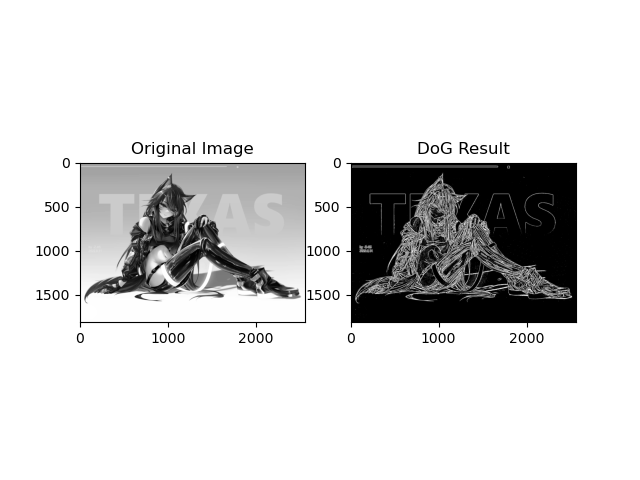
\includegraphics[width=8cm,height=5cm, keepaspectratio]{Figure_0.png} 
    \caption{DoG模型效果图}
    \label{f0}
\end{figure}
\begin{figure}[htbp]
    \centering
    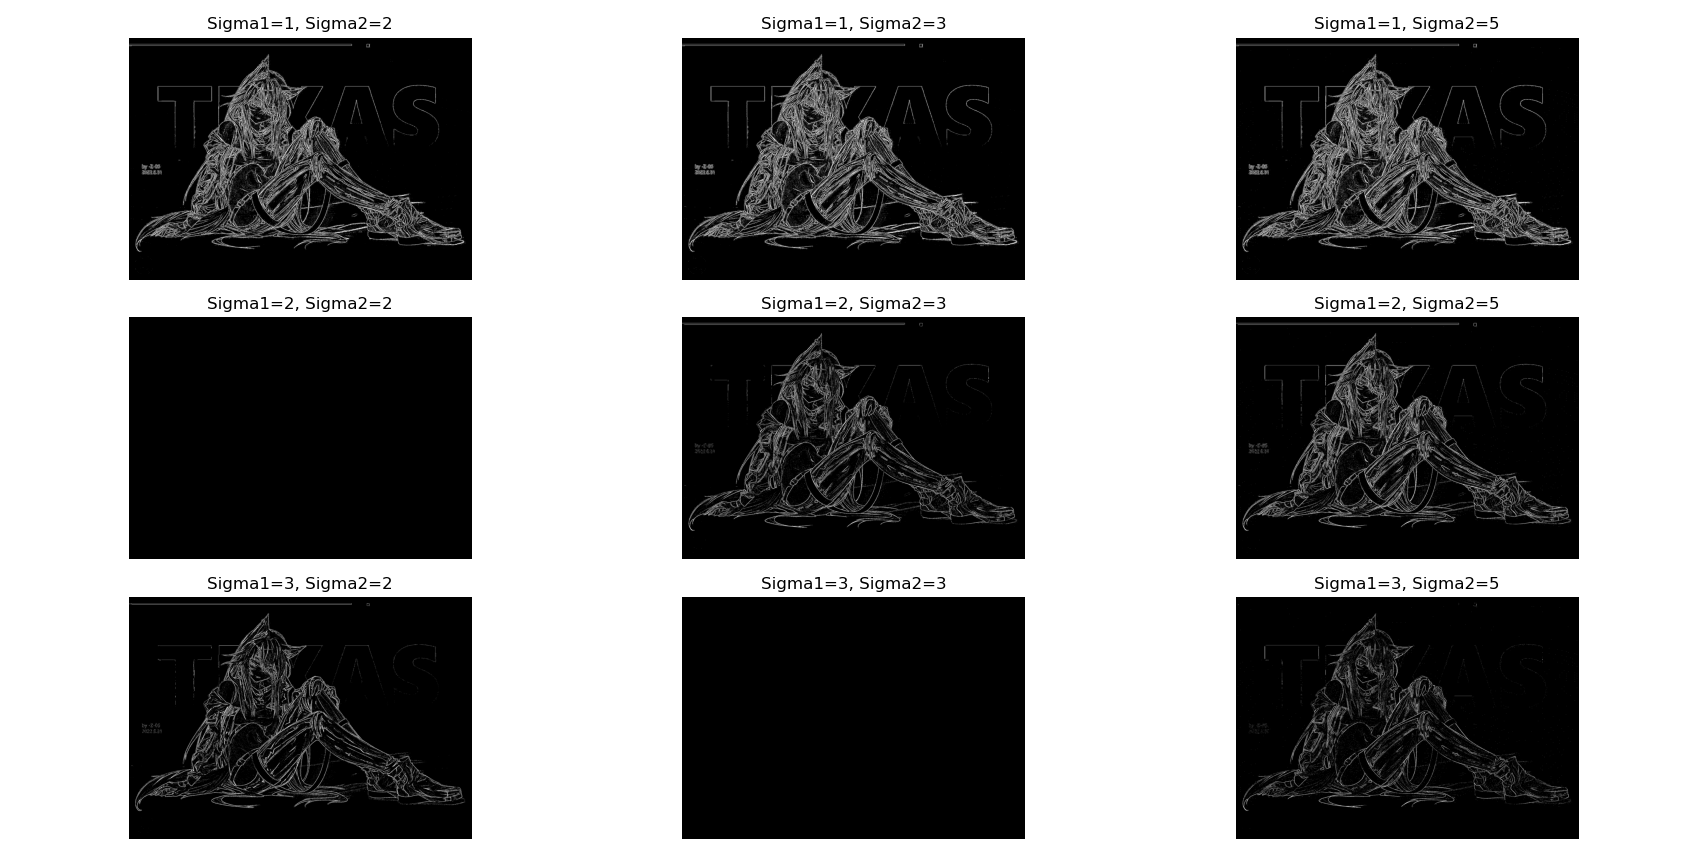
\includegraphics[width=8cm,height=5cm, keepaspectratio]{Figure_1.png} 
    \caption{不同参数下的模型效果对比}
    \label{f1}
\end{figure}
\newpage
\section{个人心得}
类脑计算是一个典型的跨学科研究领域,涉及计算机科学、神经科学、电子工程等多个学科的知识。本课程的学习让我深刻体会到不同学科之间的相互关联和协作的重要性。生物学上的发现可以直接启发新型计算架构的设计;而计算机科学的进步又能反过来推动神经科学研究的发展。这种多学科交叉不仅促进了对人脑工作原理的深入理解,还推动了新型智能系统的开发。在本课程的学习过程中,我深刻体会到不同学科之间的相互关联和协作的重要性。每个学科都为解决复杂问题提供了独特的视角和工具,而这些视角和工具的结合往往能带来意想不到的创新成果。

本人曾有幸参与视觉计算实验室承担的一项国家自然科学基金项目“疾病调控因子的异质图可视化研究分析”,专注于miRNA(微小核糖核酸)与疾病关联方向的研究。这样的研究经历让我亲身体验到了跨学科合作的魅力所在。我们利用生物信息学方法解析基因表达数据,并构建出反映miRNA与疾病之间关系的图神经网络模型。这样用计算的方式来表现RNA的结构,与类脑计算中用计算的方式来表现人脑工作机理的方法异曲同工。

正如本文的标题所说,科学界对人脑的探索仍然是关山初度路犹长,水面之下仍然有八分之七的冰山等待人们未来去发现。尽管我们已经在类脑计算、神经科学以及生物信息学等领域取得了显著进展,但相对于复杂而神秘的大脑,我们所了解的仅仅是冰山一角。随着技术的进步和跨学科合作的深化,未来的探索将更加深入,并可能带来颠覆性的突破。尽管前方的道路充满挑战,但我们有足够的理由相信,在不断前进的过程中,人类终将揭开大脑这一神秘领域的更多面纱。每一次小的进步都是向着最终目标迈进的重要一步,而跨学科的合作精神则是照亮这条漫长旅途的明灯。通过持续的努力和探索,我们不仅能够更深刻地理解自己,还能够利用这些新知造福全人类,创造一个更加美好的世界。

\printbibliography

\newpage
\section{附录}

\subsection{DoG模型实现代码:}
\begin{figure}[htbp]
    \centering
    \includegraphics[width=12cm,height=15cm, keepaspectratio]{DOG1.png} 
    
    \label{f0}
\end{figure}
\newpage
\subsection{DoG模型调参代码:}
\begin{figure}[htbp]
    \centering
    \includegraphics[width=12cm,height=15cm, keepaspectratio]{DOG2.png} 
   
    \label{f0}
\end{figure}



\end{document}